%!TEX root =../mapp-challenge-18-game-book.tex
% ^ leave for LaTeXTools build functionality

\phSection{Opening Puzzle - TODO}

TODO

\phSection{Main Puzzle 1 - Go Get 'Em}

The correct stones are laid as follows.

\begin{multicols}{3}
\begin{itemize}
  \item Black on JT - \texttt{T}
  \item White on HQ - \texttt{H}
  \item White on EZ - \texttt{E}
  \item White on FP - \texttt{F}
  \item Black on BO - \texttt{O}
  \item Black on ER - \texttt{R}
  \item White on EO - \texttt{E}
  \item Black on GS - \texttt{S}
  \item Black on ET - \texttt{T}
\end{itemize}
\end{multicols}

The solution is \texttt{THEFOREST}.

\phSection{Main Puzzle 2 - When Push Comes to Shove}



\begin{multicols}{2}
  \begin{itemize}
    \item \texttt{M=13=2+11}
      The number of ways you can stack either \(2\) or \(6\) boxes.
    \item \texttt{O=15}
      The number of ways you can stack \(12\) boxes, if every row must
      contain an odd number.
    \item \texttt{U=21=22-1}
      The number of ways you can stack \(8\) boxes, if every row must contain
      less than eight.
    \item \texttt{S=19=1+1+2+3+5+7}
      The number of ways you can stack up to \(5\) boxes. (An empty room
      counts as one way...)
    \item \texttt{E=5}
      The number of ways you can stack \(4\) boxes.
  \end{itemize}
\columnbreak
  \begin{itemize}
    \item \texttt{T=20=22-2}
      The number of ways you can stack \(8\) boxes, if every row must contain
      less than seven.
    \item \texttt{R=18}
      The number of ways you can stack \(13\) boxes, if every row must have
      less boxes than the row below it.
    \item \texttt{A=1}
      The number of ways you can stack \(42\) boxes, if you can only use one
      row.
    \item \texttt{P=16=1+15}
      The number of ways you can stack \(1\) or \(12\) boxes, if every row must
      have a unique number of boxes.
  \end{itemize}
\end{multicols}

The solution is \texttt{MOUSETRAP}.

\phSection{Main Puzzle 3 - The Name Rater}

Since vowels are always doubled or subtracted by \(3\) when creating
excellent nicknames, and the basic excellent nicknames
have exactly one vowel, it is impossible for an excellent nickname
to have a multiple of \(3\) vowels in a word.
Thus all the words that have \(3\) vowels are not excellent (and the
others can be verified to be excellent).

\begin{multicols}{2}
  \begin{itemize}
    \item \textbf{MANKAY} \texttt{4As->BA->B->BABBAB}
    \item \textit{ULTRAMON} (3 vowels)
    \item \textbf{OMASTARE} \texttt{16As->ABABBABA}
    \item \textit{VOLTEON} (3 vowels)
    \item \textit{GENGASKHAN} (3 vowels)
    \item \textit{EEVOL} (3 vowels)
    \item \textbf{NOHTYP} \texttt{16As->BABBBB}
    \item \textit{BLASTMOIST} (3 vowels)
    \item \textbf{ICHU} \texttt{8As->ABBA}
    \item \textbf{KADABARA} \texttt{4As->BA->BABABABA}
    \item \textit{AERODYCTL} (3 vowels)
    \item \textit{PARACENT} (3 vowels)
    \item \textbf{EARSEA} \texttt{16As->AABBAABB->AABBAA}
    \item \textit{DRAGONAT} (3 vowels)
    \item \textbf{RAGMAR} \texttt{4As->BA->BAB->BABBAB}
  \end{itemize}
\end{multicols}

The solution \texttt{MONIKER} is another word for nickname
(but is not excellent as a nickname, because it has 3 vowels).

\phSection{Main Puzzle 4 - An Unending Enigma}

\begin{align*}
  (\omega+3)\cdot(\omega+5)&=\omega^2\cdot E+\omega\cdot G+S
                            =\omega^2\cdot 1+\omega\cdot 5+3 \\
  \omega+1+\omega+3+\omega+5+\omega+7&=\omega\cdot I+O
                                      =\omega\cdot 4+7 \\
  3\cdot\omega+\omega^2\cdot 5+4\cdot(\omega^2+2)&=
        \omega^2\cdot L+\omega\cdot R+N =
        \omega^2\cdot 6+\omega\cdot 0+8 \\
  2\cdot(2+\omega\cdot3)+(\omega\cdot3+2)\cdot2&=
        \omega\cdot A+M =
        \omega\cdot 9+2
\end{align*}

This yields the solution \texttt{24007042951=MIRRORIMAGE}.

\phSection{Cryptic Puzzle 1 - Civic Duty}

This puzzle is solved by ordering the \mappMobimon{} alphabetically,
then converting the required number of trainers for each
using A=1,B=2, etc.

\begin{multicols}{2}
\begin{itemize}
  \item {Ayepey}: \(P=16\)
  \item {Burnie}: \(R=18\)
  \item {Corporil}: \(U=21\)
  \item {Dankgunk}: \(D=4\)
  \item {Electrumble}: \(E=5\)
  \item {Forluxi}: \(N=14\)
  \item {Glooble}: \(C=3\)
  \item {Hearit}: \(E=5\)
\end{itemize}
\end{multicols}

The solution is \texttt{PRUDENCE}.

\phSection{Cryptic Puzzle 2 - Cross Product}

``Only a trainer that has one of these can possibly become HIPCONAM.''
\texttt{HIPCONAM} is an anagram of \texttt{CHAMPION}, hinting players to
search for anagrams of the seven given words within the grid.

\begin{center}
\resizebox{2in}{!}{
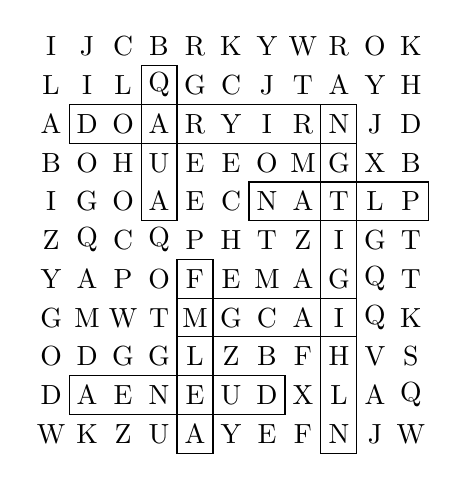
\begin{tikzpicture}[x=1.3em,y=1.4em]
  \node at (0,11) {I};\node at (1,11) {J};\node at (2,11) {C};\node at (3,11) {B};\node at (4,11) {R};\node at (5,11) {K};\node at (6,11) {Y};\node at (7,11) {W};\node at (8,11) {R};\node at (9,11) {O};\node at (10,11) {K};
  \node at (0,10) {L};\node at (1,10) {I};\node at (2,10) {L};\node at (3,10) {Q};\node at (4,10) {G};\node at (5,10) {C};\node at (6,10) {J};\node at (7,10) {T};\node at (8,10) {A};\node at (9,10) {Y};\node at (10,10) {H};
  \node at (0,9) {A};\node at (1,9) {D};\node at (2,9) {O};\node at (3,9) {A};\node at (4,9) {R};\node at (5,9) {Y};\node at (6,9) {I};\node at (7,9) {R};\node at (8,9) {N};\node at (9,9) {J};\node at (10,9) {D};
  \node at (0,8) {B};\node at (1,8) {O};\node at (2,8) {H};\node at (3,8) {U};\node at (4,8) {E};\node at (5,8) {E};\node at (6,8) {O};\node at (7,8) {M};\node at (8,8) {G};\node at (9,8) {X};\node at (10,8) {B};
  \node at (0,7) {I};\node at (1,7) {G};\node at (2,7) {O};\node at (3,7) {A};\node at (4,7) {E};\node at (5,7) {C};\node at (6,7) {N};\node at (7,7) {A};\node at (8,7) {T};\node at (9,7) {L};\node at (10,7) {P};
  \node at (0,6) {Z};\node at (1,6) {Q};\node at (2,6) {C};\node at (3,6) {Q};\node at (4,6) {P};\node at (5,6) {H};\node at (6,6) {T};\node at (7,6) {Z};\node at (8,6) {I};\node at (9,6) {G};\node at (10,6) {T};
  \node at (0,5) {Y};\node at (1,5) {A};\node at (2,5) {P};\node at (3,5) {O};\node at (4,5) {F};\node at (5,5) {E};\node at (6,5) {M};\node at (7,5) {A};\node at (8,5) {G};\node at (9,5) {Q};\node at (10,5) {T};
  \node at (0,4) {G};\node at (1,4) {M};\node at (2,4) {W};\node at (3,4) {T};\node at (4,4) {M};\node at (5,4) {G};\node at (6,4) {C};\node at (7,4) {A};\node at (8,4) {I};\node at (9,4) {Q};\node at (10,4) {K};
  \node at (0,3) {O};\node at (1,3) {D};\node at (2,3) {G};\node at (3,3) {G};\node at (4,3) {L};\node at (5,3) {Z};\node at (6,3) {B};\node at (7,3) {F};\node at (8,3) {H};\node at (9,3) {V};\node at (10,3) {S};
  \node at (0,2) {D};\node at (1,2) {A};\node at (2,2) {E};\node at (3,2) {N};\node at (4,2) {E};\node at (5,2) {U};\node at (6,2) {D};\node at (7,2) {X};\node at (8,2) {L};\node at (9,2) {A};\node at (10,2) {Q};
  \node at (0,1) {W};\node at (1,1) {K};\node at (2,1) {Z};\node at (3,1) {U};\node at (4,1) {A};\node at (5,1) {Y};\node at (6,1) {E};\node at (7,1) {F};\node at (8,1) {N};\node at (9,1) {J};\node at (10,1) {W};

  \draw (0.5,8.5) rectangle (8.5,9.5);
  \draw (2.5,6.5) rectangle (3.5,10.5);
  \draw (7.5,0.5) rectangle (8.5,9.5);
  \draw (5.5,6.5) rectangle (10.5,7.5);
  \draw (3.5,3.5) rectangle (8.5,4.5);
  \draw (3.5,0.5) rectangle (4.5,5.5);
  \draw (0.5,1.5) rectangle (6.5,2.5);
\end{tikzpicture}
}
\end{center}

Each ``cross product'' represents the letter where the two words cross in
the grid, yielding the following.

\begin{center}
Lightning \(\times\) Plant = T\hfill
Undead \(\times\) Flame = E\hfill
Aqua \(\times\) Ordinary = A\hfill
Flame \(\times\) Magic = M
\end{center}

The solution is \texttt{TEAM}.

\phSection{Cryptic Puzzle 3 - Blind Luck}

The blind/sight clues suggest to find a way to criss-cross the given
words in the grid using Braille. There is exactly one way to do this,
involving various orientations for each word.

\begin{center}
\resizebox{3in}{!}{
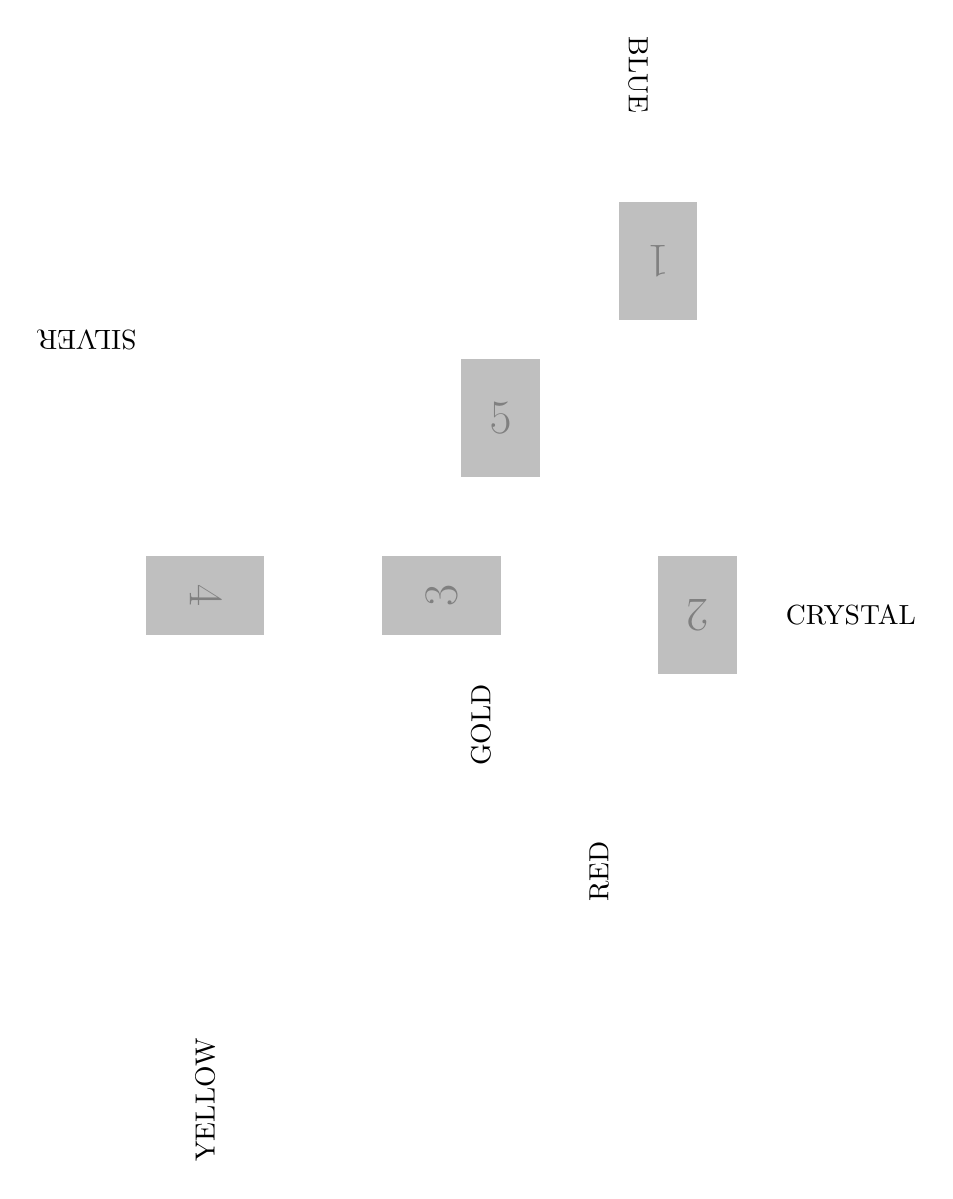
\begin{tikzpicture}[x=0.5cm,y=0.5cm]
  \fill[color=lightgray] (8,14) rectangle (10,17);
  \fill[color=lightgray] (0,10) rectangle (3,12);
  \fill[color=lightgray] (6,10) rectangle (9,12);
  \fill[color=lightgray] (13,9) rectangle (15,12);
  \fill[color=lightgray] (12,18) rectangle (14,21);

  \blindCrissCrossEntry{(0,0)}{(3,12)};
  \blindCrissCrossEntry{(2,9)}{(16,12)};
  \blindCrissCrossEntry{(10,5)}{(13,11)};
  \blindCrissCrossEntry{(7,9)}{(10,17)};
  \blindCrissCrossEntry{(0,16)}{(12,19)};
  \blindCrissCrossEntry{(11,15)}{(14,23)};

  %YELLOW
  \node[anchor=north] at (1.5,0) {\rotatebox{90}{YELLOW}};

  \blindCrissCrossPip{0}{0};
  \blindCrissCrossPip{2}{0};

  \blindCrissCrossPip{0}{1};
  \blindCrissCrossPip{1}{1};
  \blindCrissCrossPip{2}{1};

  \blindCrissCrossPip{0}{2};

  \blindCrissCrossPip{1}{3};

  \blindCrissCrossPip{0}{4};
  \blindCrissCrossPip{1}{4};
  \blindCrissCrossPip{2}{4};

  \blindCrissCrossPip{0}{6};
  \blindCrissCrossPip{1}{6};
  \blindCrissCrossPip{2}{6};

  \blindCrissCrossPip{0}{8};
  \blindCrissCrossPip{2}{8};

  \blindCrissCrossPip{1}{9};

  \blindCrissCrossPip{1}{10};

  \blindCrissCrossPip{0}{11};
  \blindCrissCrossPip{1}{11};
  \blindCrissCrossPip{2}{11};

  %CRYSTAL
  \node[anchor=west] at (16,10.5) {CRYSTAL};
  \blindCrissCrossPip{2}{11};

  \blindCrissCrossPip{3}{11};

  \blindCrissCrossPip{4}{9};
  \blindCrissCrossPip{4}{10};
  \blindCrissCrossPip{4}{11};

  \blindCrissCrossPip{5}{10};

  \blindCrissCrossPip{6}{9};
  \blindCrissCrossPip{6}{11};

  \blindCrissCrossPip{7}{9};
  \blindCrissCrossPip{7}{10};
  \blindCrissCrossPip{7}{11};

  \blindCrissCrossPip{8}{9};
  \blindCrissCrossPip{8}{10};

  \blindCrissCrossPip{9}{11};

  \blindCrissCrossPip{10}{9};
  \blindCrissCrossPip{10}{10};

  \blindCrissCrossPip{11}{10};
  \blindCrissCrossPip{11}{11};

  \blindCrissCrossPip{12}{11};

  \blindCrissCrossPip{14}{9};
  \blindCrissCrossPip{14}{10};
  \blindCrissCrossPip{14}{11};

  %RED
  \node[anchor=north] at (11.5,5) {\rotatebox{90}{RED}};

  \blindCrissCrossPip{10}{5};
  \blindCrissCrossPip{11}{5};
  \blindCrissCrossPip{12}{5};

  \blindCrissCrossPip{11}{6};

  \blindCrissCrossPip{10}{7};

  \blindCrissCrossPip{11}{8};

  \blindCrissCrossPip{10}{9};

  \blindCrissCrossPip{10}{10};
  \blindCrissCrossPip{11}{10};

  %GOLD
  \node[anchor=north] at (8.5,9) {\rotatebox{90}{GOLD}};

  \blindCrissCrossPip{7}{9};
  \blindCrissCrossPip{8}{9};

  \blindCrissCrossPip{7}{10};
  \blindCrissCrossPip{8}{10};

  \blindCrissCrossPip{7}{11};
  \blindCrissCrossPip{9}{11};

  \blindCrissCrossPip{8}{12};

  \blindCrissCrossPip{7}{13};
  \blindCrissCrossPip{8}{13};
  \blindCrissCrossPip{9}{13};

  \blindCrissCrossPip{7}{15};

  \blindCrissCrossPip{7}{16};
  \blindCrissCrossPip{8}{16};

  %SILVER
  \node[anchor=east] at (0,17.5) {\rotatebox{180}{SILVER}};

  \blindCrissCrossPip{11}{18};
  \blindCrissCrossPip{11}{17};

  \blindCrissCrossPip{10}{16};

  \blindCrissCrossPip{9}{17};

  \blindCrissCrossPip{8}{16};

  \blindCrissCrossPip{7}{18};
  \blindCrissCrossPip{7}{17};
  \blindCrissCrossPip{7}{16};

  \blindCrissCrossPip{5}{18};
  \blindCrissCrossPip{5}{17};
  \blindCrissCrossPip{5}{16};

  \blindCrissCrossPip{4}{18};

  \blindCrissCrossPip{3}{16};

  \blindCrissCrossPip{2}{17};

  \blindCrissCrossPip{1}{18};
  \blindCrissCrossPip{1}{17};
  \blindCrissCrossPip{1}{16};

  \blindCrissCrossPip{0}{17};

  %BLUE
  \node[anchor=south] at (12.5,23) {\rotatebox{-90}{BLUE}};

  \blindCrissCrossPip{12}{22};
  \blindCrissCrossPip{13}{22};

  \blindCrissCrossPip{11}{20};
  \blindCrissCrossPip{12}{20};
  \blindCrissCrossPip{13}{20};

  \blindCrissCrossPip{11}{18};
  \blindCrissCrossPip{13}{18};

  \blindCrissCrossPip{11}{17};

  \blindCrissCrossPip{13}{16};

  \blindCrissCrossPip{12}{15};

  \node at (9,15.5) {\LARGE\rotatebox{0}{\textcolor{gray}{5}}};
  \node at (1.5,11) {\LARGE\rotatebox{-90}{\textcolor{gray}{4}}};
  \node at (7.5,11) {\LARGE\rotatebox{90}{\textcolor{gray}{3}}};
  \node at (14,10.5) {\LARGE\rotatebox{180}{\textcolor{gray}{2}}};
  \node at (13,19.5) {\LARGE\rotatebox{180}{\textcolor{gray}{1}}};
\end{tikzpicture}
}
\end{center}

The numbered regions yield \texttt{12345=ULTRA} in Braille.

\phSection{Cryptic Puzzle 4 - Pin It Down}

Overlaying the mirror images of the monsters reveals a message using
the Pig Pen cipher (where the open circles represent no dot, and the
filled-in circles represent a dot).

\begin{center}
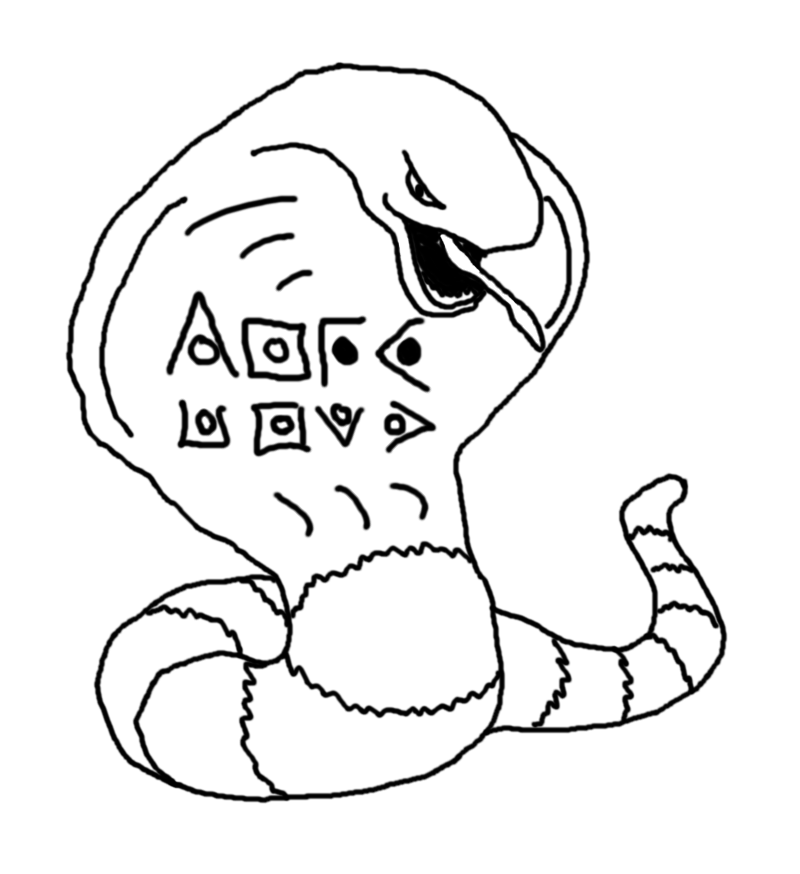
\includegraphics[width=0.3\linewidth]{assets/not-arbok-solution.png}
\end{center}

The solution is \texttt{VERYBEST}.

\phSection{Metapuzzle - The Ultimate Quartet}

TODO: complete meta and write up solution

\phSection{Hidden Puzzle}

Each of the Roads referenced in Main Puzzles 1-4, the Bonus Puzzle,
and Cryptic Puzzles 1-4 approximate to an integer between 1 and 26.

\begin{multicols}{3}
\begin{itemize}
  \item \(4.139\pi\approx13=M\)
  \item \(\sqrt{9^2+12^2}=15=O\)
  \item \(20.7183-e\approx18=R\)
  \item \(\frac{6.4984}{\sin(20^\circ)}\approx19=S\)
  \item \(6+i^2=5=E\)
  \item \(\ln(148.45)\approx5=E\)
  \item \(\tan(87.4094^\circ)\approx25=Y\)
  \item \(500\%=5=E\)
  \item \(\frac{19!}{18!}=19=S\)
\end{itemize}
\end{multicols}

\texttt{MORSEEYES} is not the solution, but a hint on how to find it.
TODO: add special accents to Mobi prefixes throughout some part of the
document available to players, spelling a solution in Morse code.

%%% Local Variables:
%%% mode: latex
%%% TeX-master: "../mapp-hsc17-game-book"
%%% End:
